\documentclass [blue] {beamer}
\usepackage{beamerthemesplit}
\usetheme{Boadilla}
%\usecolortheme{orchid}
\setbeamertemplate{footline}[text line]{}
\usepackage [latin1] {inputenc}
\usepackage [T1] {fontenc}
\usepackage [french] {babel}
\usepackage {indentfirst}
%\usepackage {graphicx}
\usepackage {geometry}
\usepackage{verbatim}
%% The amssymb package provides various useful mathematical symbols
\usepackage{amssymb}
%% The amsthm package provides extended theorem environments
%\usepackage{amsthm}
\usepackage{amsmath}
\usepackage{enumerate}
\newtheorem{proposition}[theorem]{Proposition}
\usepackage{empheq}
\usepackage{hyperref}
\hypersetup{colorlinks, citecolor=blue,%
    filecolor=blue,%
    linkcolor=blue,%
    urlcolor=blue}
%\setbeamertemplate{blocks}[shadow=false]
\setbeamercovered{transparent}
\defbeamertemplate*{footline}{my theme}
{
 \leavevmode
  \hbox{
  \begin{beamercolorbox}[wd=1\paperwidth,ht=2.25ex,dp=1ex,right,ignorebg]{date in head/foot}    \usebeamerfont{date in head/foot}\insertshortdate{}\hspace*{2em}
 S�ance 12/    \insertframenumber{} \hspace*{4ex}
  \end{beamercolorbox}}%
  \vskip0pt%
}
\usepackage{color}

\date{20 f�vrier 2014}

\title{S�ance 12 \\ Le march� du travail}
\author{Olivia D'Aoust\\
odaoust@ulb.ac.be}
\begin{document}

\frame{\titlepage}


\frame{
\frametitle{L'offre, la demande et le salaire d'�quilibre}
 
\begin{enumerate}
\item Entreprises : Demande de travail 
\item Consommateurs : Offre de travail
\end{enumerate}
\begin{center}
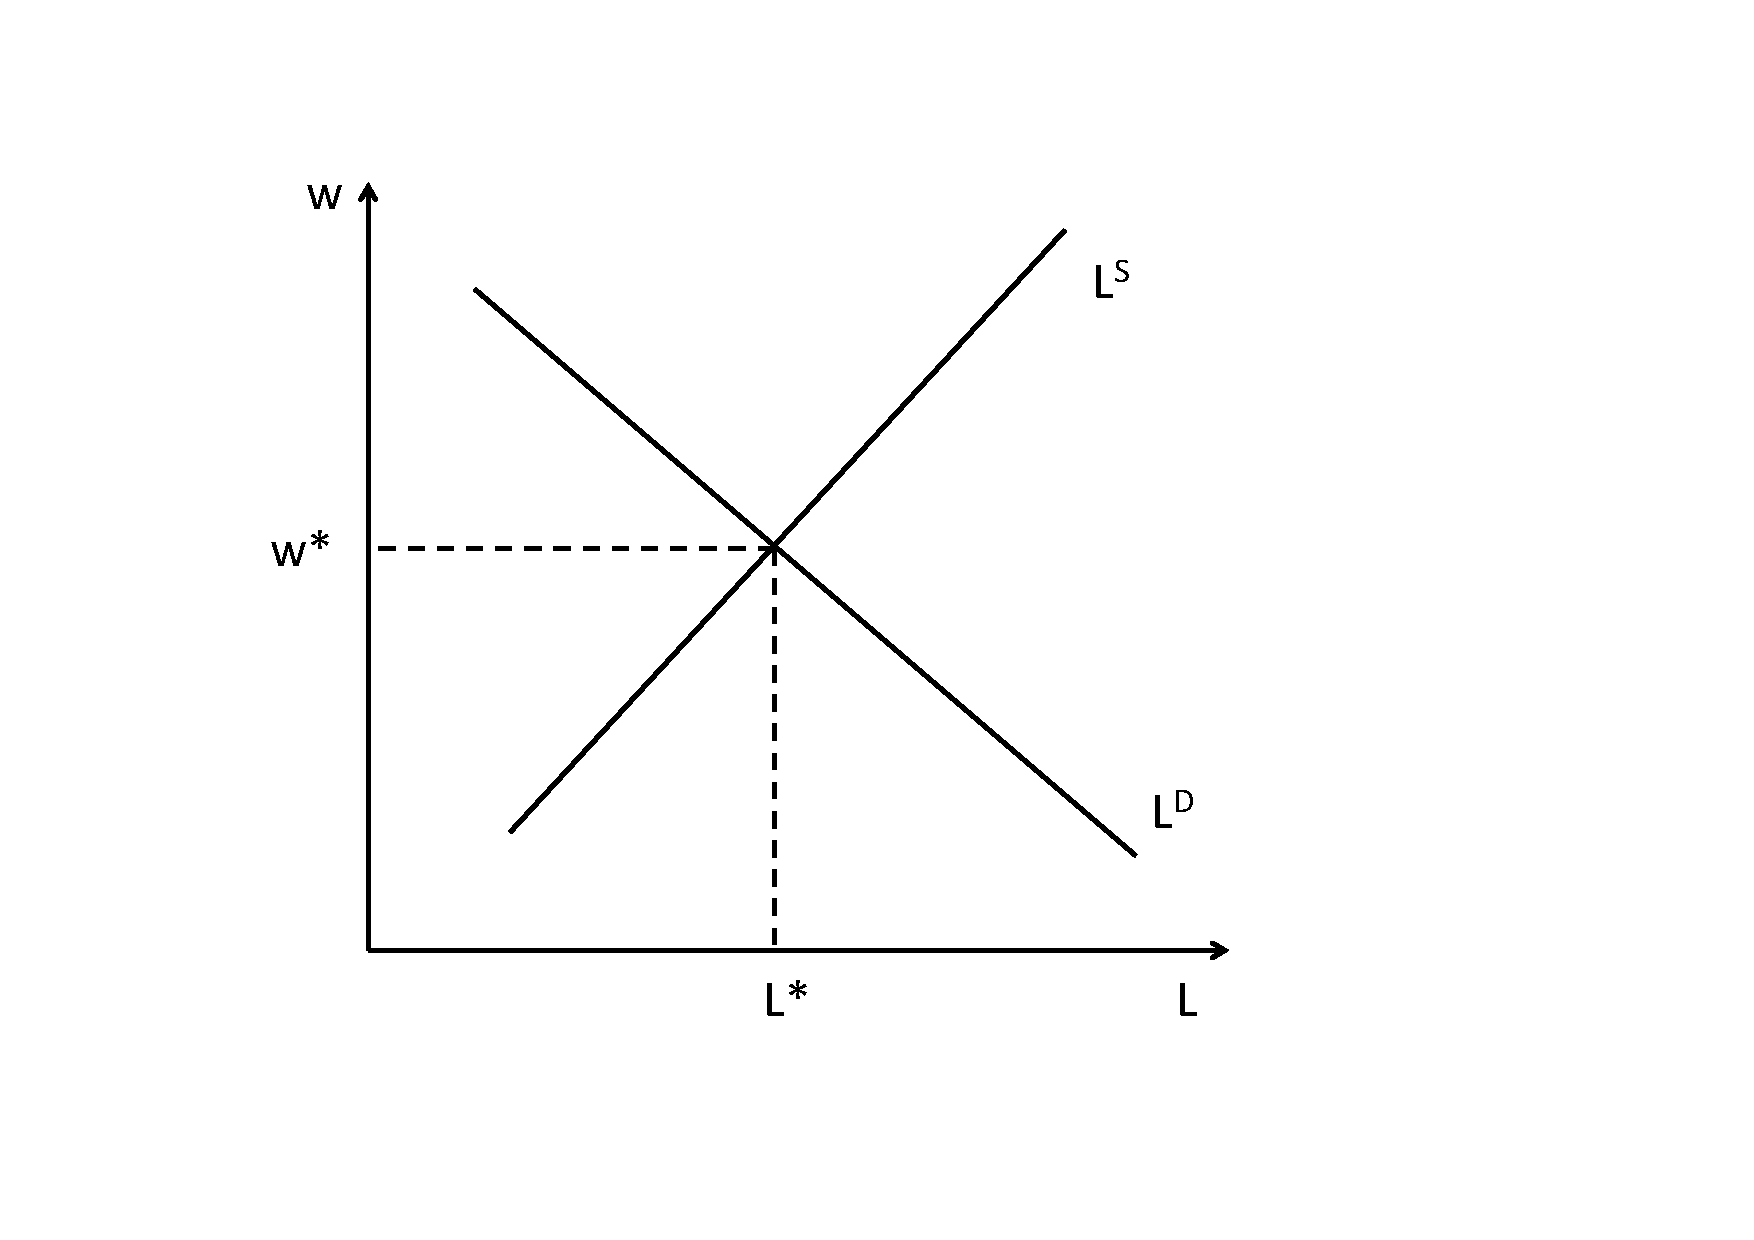
\includegraphics[trim = 3cm 4cm 3cm 2cm, scale=0.4]{mt.pdf}
\end{center}
}

\begin{frame}[allowframebreaks]
\frametitle{Demande de travail}

Rappel : la fonction de production d�crit la relation entre les inputs utilis�s pour produire et les outputs issus de la production. \\[0.3cm]

Consid�rons \textbf{la main d'oeuvre} comme \underline{seul} input endog�ne (les autres inputs (Capital, Terrain) sont fixes)\\[0.3cm]

La fonction de production est not�e f(L). \\[0.3cm]

La fonction de production est croissante (f'(L) $>$0), et concave (f''(L) $<$ 0)
%\vspace{-0.2cm}
\begin{columns}
\begin{column}[l]{5cm}
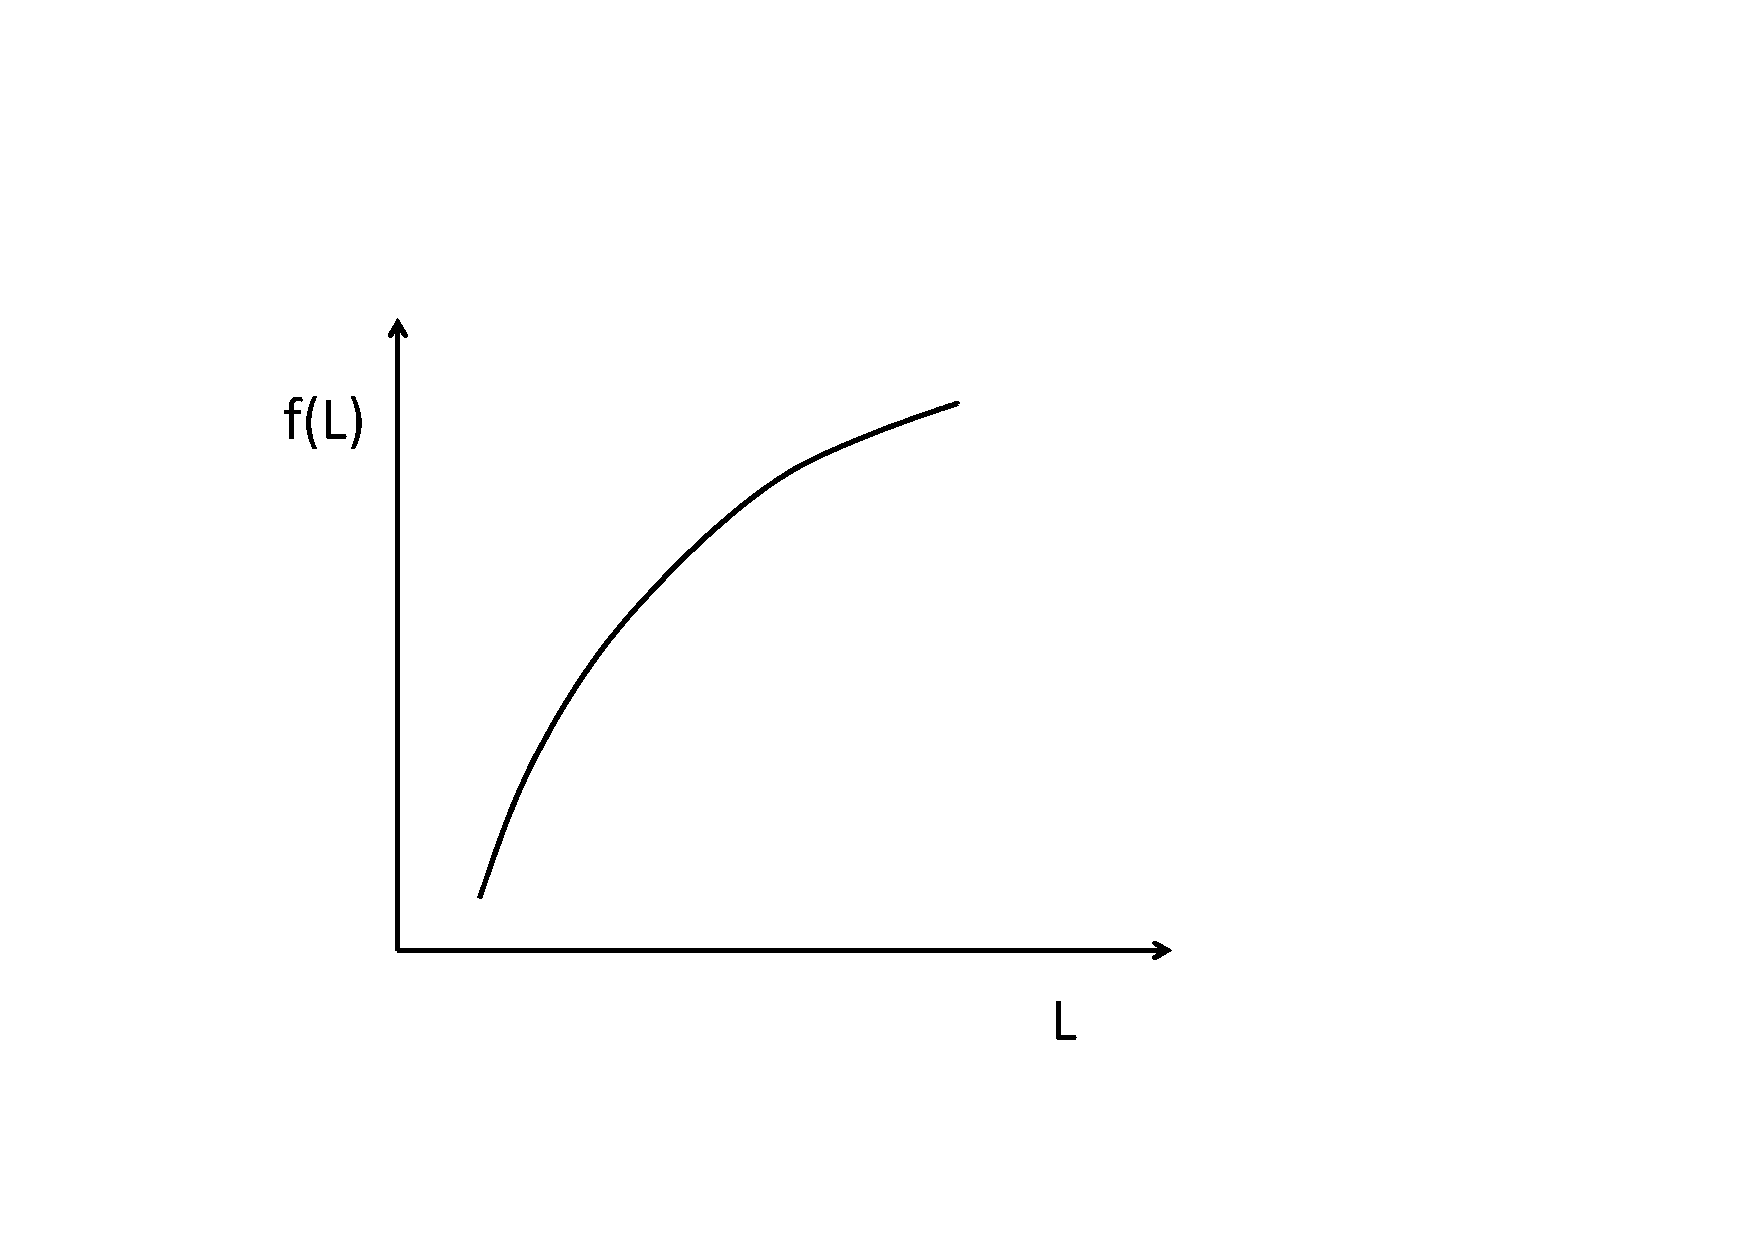
\includegraphics[clip=true,trim = 4cm 2cm 6cm 3.5cm,scale=0.25]{f.pdf}
\end{column}
\begin{column}[l]{7cm}
La quantit� produite par travailleur additionnel que l'entreprise engage diminue lorsque le nombre de travailleurs augmente: \textbf{rendements marginaux d�croissants}\\[0.2cm]
\emph{Exemple : production de pommes}
\end{column}
\end{columns}

\break

L'entreprise choisit la demande de travail qui maximise son profit : la diff�rence entre ses revenus (prix $\times$ quantit�) et ses co�ts (nr. de travailleurs $\times$ salaire par travailleur)

\begin{equation}\nonumber
\max_L \pi = p f(L) -  w L
\end{equation}

\begin{equation}\nonumber
\frac{\partial \pi}{\partial L} = 0 \rightarrow p f'(L) - w = 0
\end{equation}

\begin{equation}\nonumber
\underbrace{w}_{\text{\parbox{6em}{ Co�t par travailleur}}} = \underbrace{p f'(L)}_{\text{\parbox{6em}{Revenu par travailleur}}}
\end{equation}
\begin{center}
salaire nominal = productivit� marginale en valeur
\end{center}

\break

\begin{center}
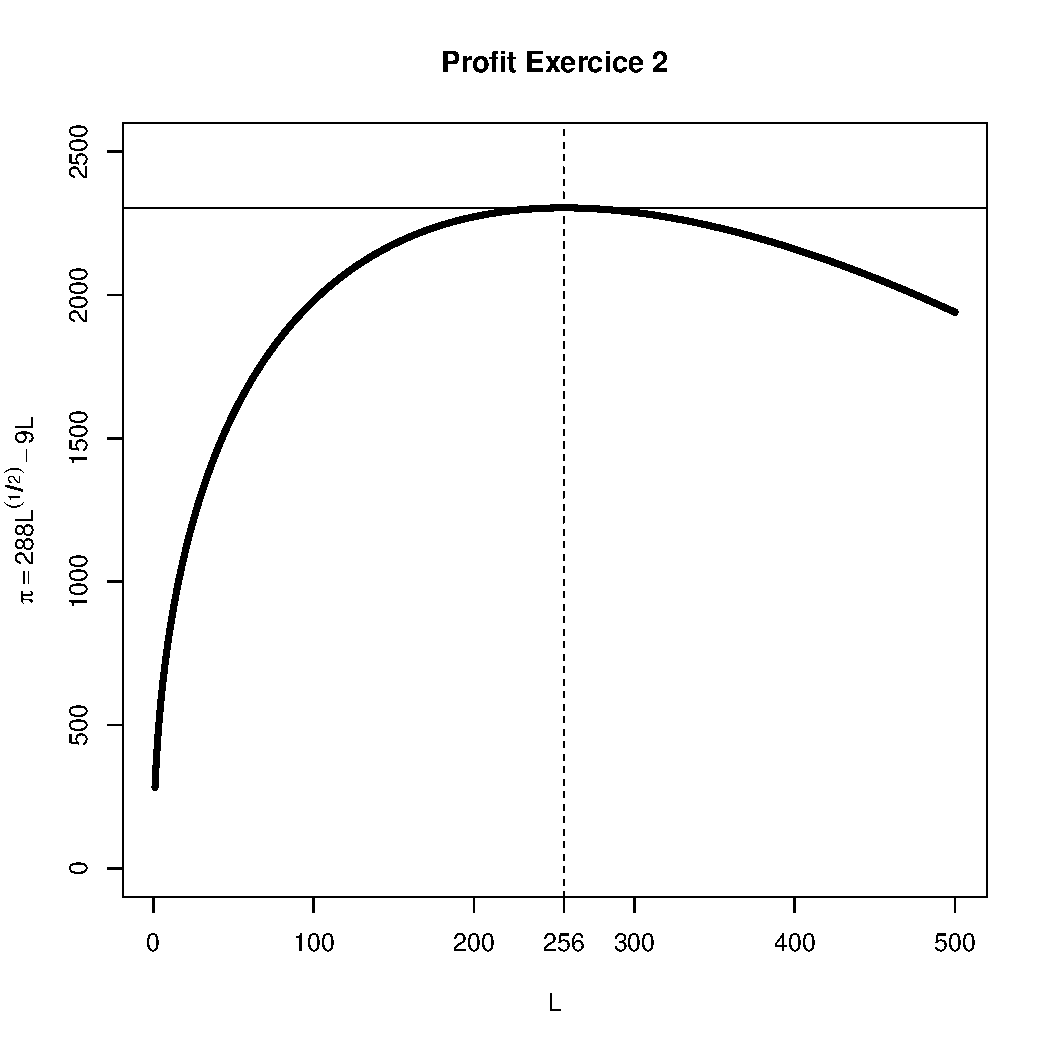
\includegraphics[scale=0.5]{ex2.pdf}
 \end{center}

\end{frame}

\frame{
\frametitle{Demande de travail IV}

\begin{columns}
\begin{column}[l]{6cm}
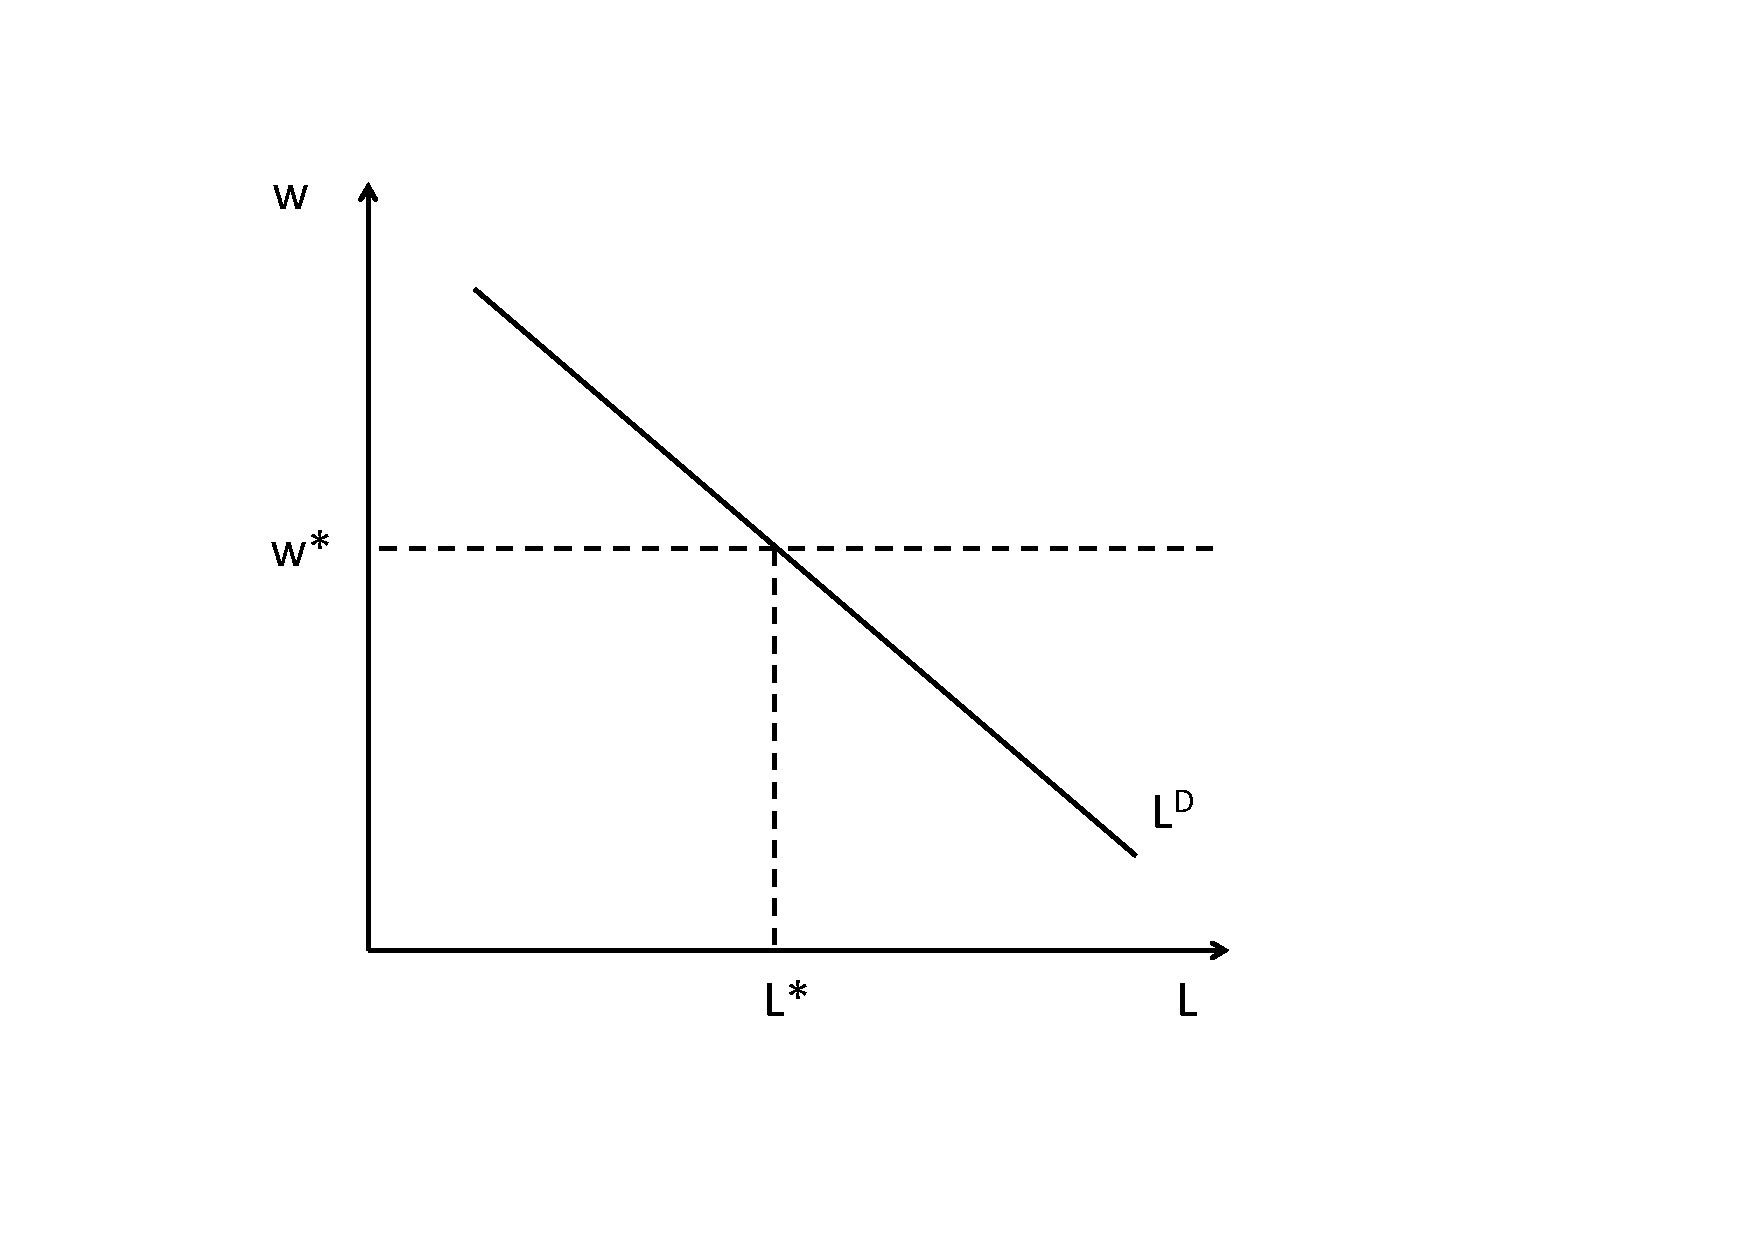
\includegraphics[clip=true,trim = 4cm 3cm 7cm 2cm,scale=0.32]{dem.pdf}
\end{column}
\begin{column}[l]{6cm}
La demande de main d'oeuvre optimale veut que 
\begin{equation}\nonumber
w = p f'(L) 
\end{equation}

$\rightarrow$ le salaire est �gal � la productivit� marginale en valeur\\[0.3cm]

$f''(L) < 0$ indique que la productivit� marginale (f'(L)) est une fonction d�croissante en L.\\[0.3cm]
 Lorsque L augmente, $f'(L)$ diminue, et w diminue selon $w = p f'(L)$ car $p > 0$

\end{column}
\end{columns}
}

\frame{
\frametitle{Offre de travail}
\begin{columns}
\begin{column}[l]{6cm}
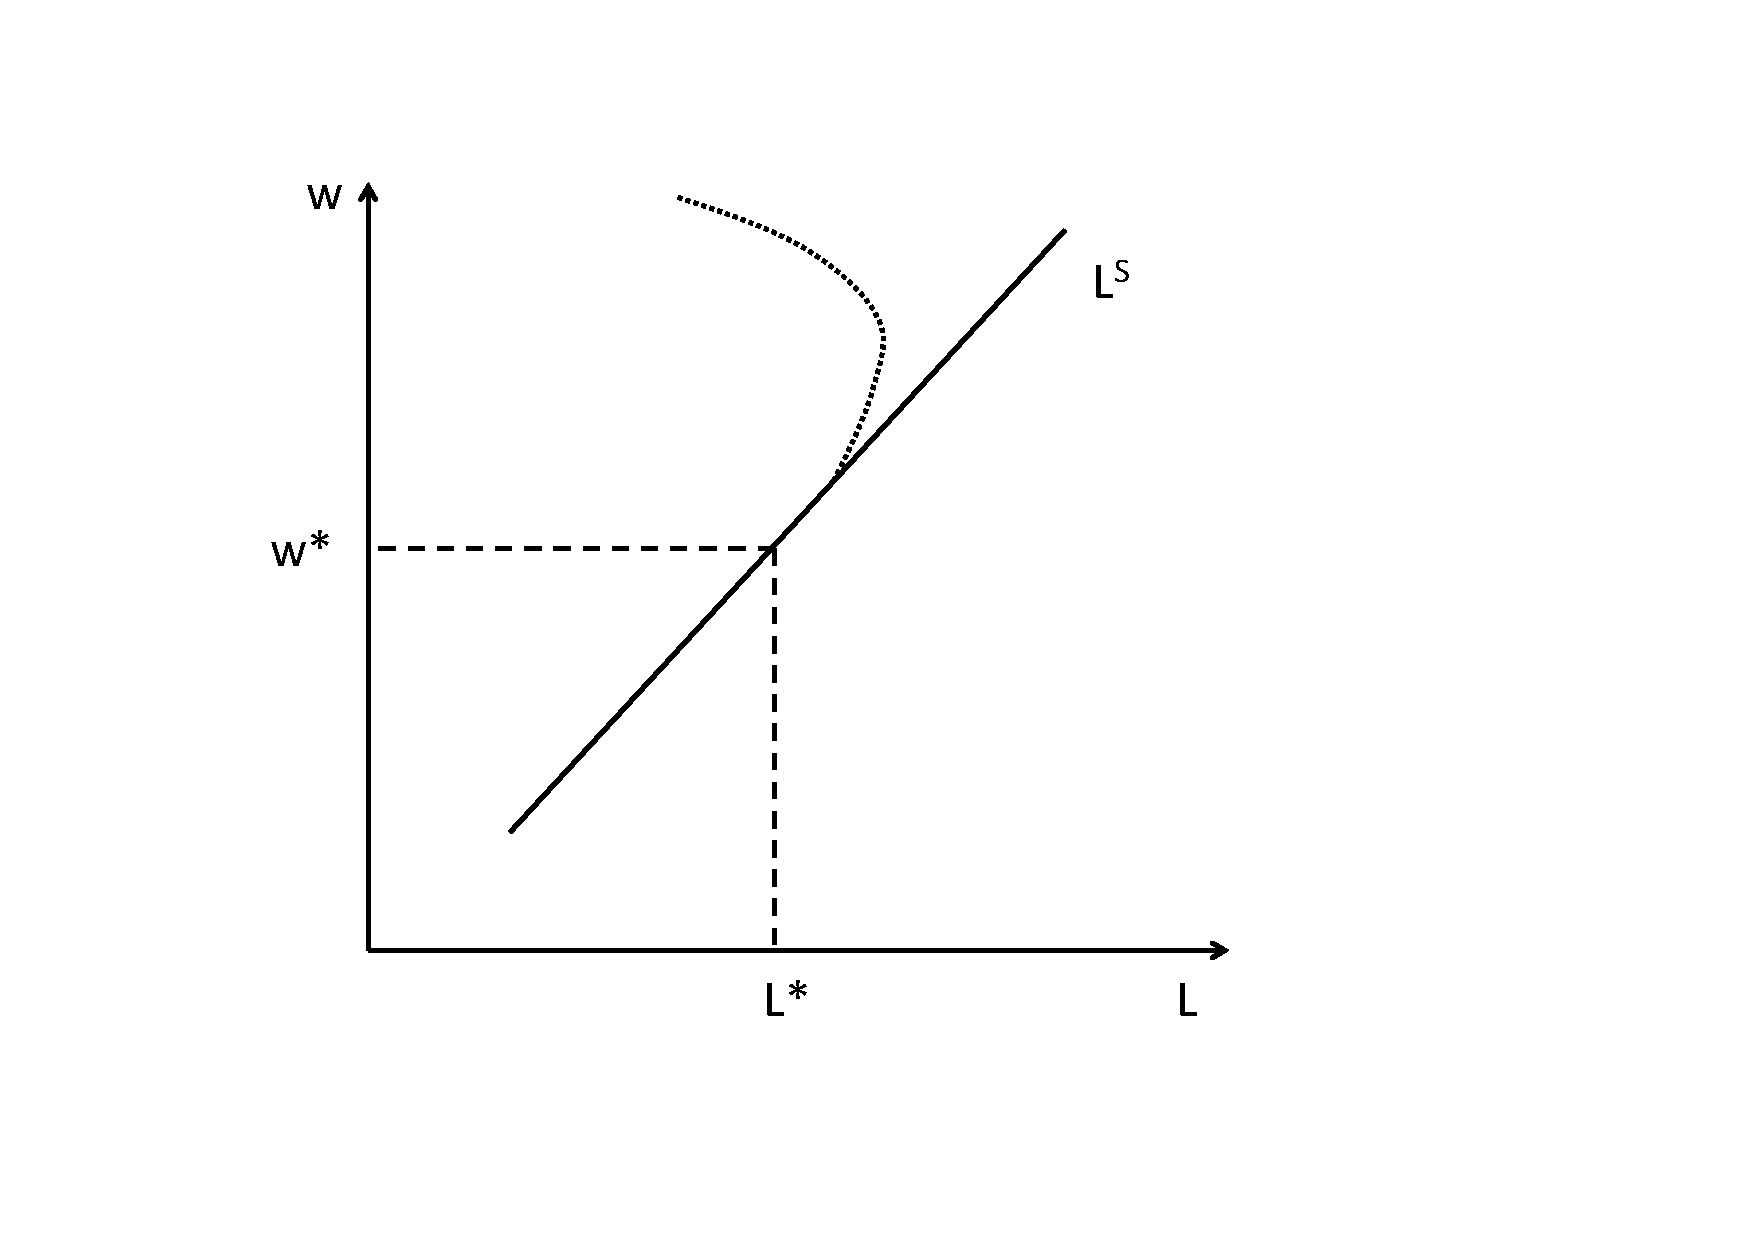
\includegraphics[clip=true,trim = 4cm 3cm 7cm 2cm,scale=0.32]{offre.pdf}
\end{column}
\begin{column}[l]{6cm}
Lorsque le salaire w augmente, on distingue deux effets:
\begin{itemize}
\item l'effet substitution : $\Delta^+$ w augmente le co�t d'opportunit� du loisir, et implique $\Delta^+$ L 
\item l'effet revenu : $\Delta^+$ w implique que l'on peut travailler moins pour gagner autant, et implique $\Delta^-$ L 
\end{itemize}

\end{column}
\end{columns}

}


\frame{
\frametitle{Exercices suppl�mentaires}

\textbf{Exercice 7}

Les propositions a), b), c) et d) sont correctes \\[0.3cm]

\textbf{Exercice 8}

Les propositions a), b) sont correctes \\[0.3cm]


\textbf{Exercice 9}

La proposition e) est correcte \\[0.3cm]


\textbf{Exercice 10}

Les propositions b), d), e) l) et m) sont correctes \\[0.3cm]



}


\end{document}